%%%%%%%%%%%%%%%%%%%%%%%%%%%%%%%%%%%%%%%%%
% Classicthesis Typographic Thesis
% LaTeX Template
% Version 1.3 (15/2/14)
%
% This template has been downloaded from:
% http://www.LaTeXTemplates.com
%
% Original author:
% André Miede (http://www.miede.de)
%
% License:
% CC BY-NC-SA 3.0 (http://creativecommons.org/licenses/by-nc-sa/3.0/)
%
% General Tips:
% 1) Make sure to edit the classicthesis-config.file
% 2) New enumera tion (A., B., C., etc in small caps): \begin{aenumerate} \end{aenumerate}
% 3) For margin notes: \marginpar or \graffito{}
% 4) Do not use bold fonts in this style, it is designed around them
% 5) Use tables as in the examples
% 6) See classicthesis-preamble.sty for useful commands
%
%%%%%%%%%%%%%%%%%%%%%%%%%%%%%%%%%%%%%%%%%

%----------------------------------------------------------------------------------------
%	PACKAGES AND OTHER DOCUMENT CONFIGURATIONS
%----------------------------------------------------------------------------------------
\documentclass[
		twoside,titlepage,numbers=noenddot,headinclude,%1headlines, titlepage openleft
                footinclude=true,cleardoublepage=empty,
                fontsize=9pt, %paper=a4,  BCOR=5mm,% Binding correction, paper type and font size BCOR=5mm,
                ngerman,american, % Languages
                ]{scrreprt} 
 
                
% Includes the file which contains all the document configurations and packages - make sure to edit this file
%%%%%%%%%%%%%%%%%%%%%%%%%%%%%%%%%%%%%%%%%
% Thesis Configuration File
%
% The main lines to change in this file are in the DOCUMENT VARIABLES
% section, the rest of the file is for advanced configuration.
%
%%%%%%%%%%%%%%%%%%%%%%%%%%%%%%%%%%%%%%%%%



%----------------------------------------------------------------------------------------
%	DOCUMENT VARIABLES
%	Fill in the lines below to enter your information into the thesis template
%	Each of the commands can be cited anywhere in the thesis
%----------------------------------------------------------------------------------------

% Remove drafting to get rid of the '[ Date - classicthesis version 4.0 ]' text at the bottom of every page
\PassOptionsToPackage{eulerchapternumbers, pdfspacing,  subfig, linedheaders, subfig,beramono,eulermath,floatperchapter,manychapters}{classicthesis}
% Available options: drafting parts nochapters linedheaders eulerchapternumbers beramono eulermath pdfspacing minionprospacing tocaligned dottedtoc manychapters listings floatperchapter subfig
% Adding 'dottedtoc' will make page numbers in the table of contents flushed right with dots leading to them
% lineheaders have been modified to not have the line above -20180220 see sty file line 373.
% floatperchapter makes figures numbering uniform and not connected with chapter numbers

\newcommand{\myTitle}{Main Title goes here \xspace}
\newcommand{\mySubtitle}{Subtitle goes here\xspace} % desining safe workstatons for smooth operations
\newcommand{\myDegree}{Doktorand\xspace}
\newcommand{\myName}{ChatGPT 3.5\xspace}
\newcommand{\myProf}{Supervisor - 1\xspace}
\newcommand{\myOtherProf}{Supervisor - 1 \xspace}
\newcommand{\mySupervisor}{Supervisor - 1\xspace}
\newcommand{\myFaculty}{Division of Machine Design\xspace}
\newcommand{\myDepartment}{Department of Management and Engineering\xspace}
\newcommand{\myUni}{Link\"{o}ping University\xspace}
\newcommand{\myLocation}{Link\"{o}ping, Sweden\xspace}
\newcommand{\myTime}{December 2019\xspace}
\newcommand{\myVersion}{xxxx\xspace}

%----------------------------------------------------------------------------------------
%	USEFUL COMMANDS
%----------------------------------------------------------------------------------------

\newcommand{\ie}{i.\,e.}
\newcommand{\Ie}{I.\,e.}
\newcommand{\eg}{e.\,g.}
\newcommand{\Eg}{E.\,g.} 

\newcounter{dummy} % Necessary for correct hyperlinks (to index, bib, etc.)
\providecommand{\mLyX}{L\kern-.1667em\lower.25em\hbox{Y}\kern-.125emX\@}



%----------------------------------------------------------------------------------------
%	PACKAGES
%----------------------------------------------------------------------------------------

\usepackage{lipsum} % Used for inserting dummy 'Lorem ipsum' text into the template

%------------------------------------------------
 
%\PassOptionsToPackage{latin9}{inputenc} % latin9 (ISO-8859-9) = latin1+"Euro sign"
%\usepackage{inputenc}
 
 %------------------------------------------------

%\PassOptionsToPackage{ngerman,american}{babel}  % Change this to your language(s)
% Spanish languages need extra options in order to work with this template
%\PassOptionsToPackage{spanish,es-lcroman}{babel}
\usepackage{babel}

%------------------------------------------------			

%\PassOptionsToPackage{sort&compress,numbers,super}{natbib}
\PassOptionsToPackage{sort&compress,numbers,square}{natbib}
 \usepackage{natbib}

 %------------------------------------------------

\PassOptionsToPackage{fleqn}{amsmath} % Math environments and more by the AMS 
 \usepackage{amsmath}
 
 %------------------------------------------------

\PassOptionsToPackage{T1}{fontenc} % T2A for cyrillics
\usepackage{fontenc}

%------------------------------------------------

\usepackage{xspace} % To get the spacing after macros right

%------------------------------------------------

\usepackage{mparhack} % To get marginpar right

%------------------------------------------------

\usepackage{fixltx2e} % Fixes some LaTeX stuff 

%------------------------------------------------

\PassOptionsToPackage{smaller}{acronym} % Include printonlyused in the first bracket to only show acronyms used in the text
\usepackage{acronym} % nice macros for handling all acronyms in the thesis

%------------------------------------------------

%\renewcommand*{\acsfont}[1]{\textssc{#1}} % For MinionPro
%\renewcommand{\bflabel}[1]{{#1}\hfill} % Fix the list of acronyms

%------------------------------------------------

\PassOptionsToPackage{pdftex}{graphicx}
\usepackage{graphicx} 
%\usepackage{subcaption}

%----------------------------------------------------------------------------------------
%	FLOATS: TABLES, FIGURES AND CAPTIONS SETUP
%----------------------------------------------------------------------------------------

\usepackage{tabularx} % Better tables
\setlength{\extrarowheight}{3pt} % Increase table row height
\newcommand{\tableheadline}[1]{\multicolumn{1}{c}{\spacedlowsmallcaps{#1}}}
\newcommand{\myfloatalign}{\centering} % To be used with each float for alignment
\usepackage{caption}
\captionsetup{format=plain,font=small,indention=.25cm} % changed format=hang and added indention=.25cm
\usepackage{subfig}  

%----------------------------------------------------------------------------------------
%	CODE LISTINGS SETUP
%----------------------------------------------------------------------------------------

\usepackage{listings} 
%\lstset{emph={trueIndex,root},emphstyle=\color{BlueViolet}}%\underbar} % for special keywords
\lstset{language=[LaTeX]Tex, % Specify the language for listings here
keywordstyle=\color{RoyalBlue}, % Add \bfseries for bold
basicstyle=\small\ttfamily, % Makes listings a smaller font size and a different font
%identifierstyle=\color{NavyBlue}, % Color of text inside brackets
commentstyle=\color{Green}\ttfamily, % Color of comments
stringstyle=\rmfamily, % Font type to use for strings
numbers=left, % Change left to none to remove line numbers
numberstyle=\scriptsize, % Font size of the line numbers
stepnumber=5, % Increment of line numbers
numbersep=8pt, % Distance of line numbers from code listing
showstringspaces=false, % Sets whether spaces in strings should appear underlined
breaklines=true, % Force the code to stay in the confines of the listing box
%frameround=ftff, % Uncomment for rounded frame
frame=single, % Frame border - none/leftline/topline/bottomline/lines/single/shadowbox/L
belowcaptionskip=.75\baselineskip % Space after the "Listing #: Desciption" text and the listing box
}

%----------------------------------------------------------------------------------------
%	HYPERREFERENCES
%----------------------------------------------------------------------------------------

\PassOptionsToPackage{pdftex,hyperfootnotes=false,pdfpagelabels}{hyperref}
\usepackage{hyperref}  % backref linktocpage pagebackref
\pdfcompresslevel=9
\pdfadjustspacing=1

\hypersetup{
% Uncomment the line below to remove all links (to references, figures, tables, etc)
%draft, 
%colorlinks=true, linktocpage=true, pdfstartpage=3, pdfstartview=FitV,
% Uncomment the line below if you want to have black links (e.g. for printing black and white)
colorlinks=false, linktocpage=true, pdfborder={0 0 0}, pdfstartpage=3, pdfstartview=FitV, 
breaklinks=true, pdfpagemode=UseNone, pageanchor=true, pdfpagemode=UseOutlines,
plainpages=false, bookmarksnumbered, bookmarksopen=true, bookmarksopenlevel=1,
hypertexnames=true, pdfhighlight=/O, urlcolor=webbrown, linkcolor=RoyalBlue, citecolor=webgreen,
%------------------------------------------------
% PDF file meta-information
pdftitle={\myTitle},
pdfauthor={\textcopyright\ \myName, \myUni, \myFaculty},
pdfsubject={},
pdfkeywords={},
pdfcreator={pdfLaTeX},
pdfproducer={LaTeX with hyperref and classicthesis}
%------------------------------------------------
}





%----------------------------------------------------------------------------------------
%	BACKREFERENCES
%----------------------------------------------------------------------------------------

\usepackage{ifthen} % Allows the user of the \ifthenelse command
\newboolean{enable-backrefs} % Variable to enable backrefs in the bibliography
\setboolean{enable-backrefs}{false} % Variable value: true or false

\newcommand{\backrefnotcitedstring}{\relax} % (Not cited.)
\newcommand{\backrefcitedsinglestring}[1]{(Cited on page~#1.)}
\newcommand{\backrefcitedmultistring}[1]{(Cited on pages~#1.)}
\ifthenelse{\boolean{enable-backrefs}} % If backrefs were enabled
{
\PassOptionsToPackage{hyperpageref}{backref}
\usepackage{backref} % to be loaded after hyperref package 
\renewcommand{\backreftwosep}{ and~} % separate 2 pages
\renewcommand{\backreflastsep}{, and~} % separate last of longer list
\renewcommand*{\backref}[1]{}  % disable standard
\renewcommand*{\backrefalt}[4]{% detailed backref
\ifcase #1 
\backrefnotcitedstring
\or
\backrefcitedsinglestring{#2}
\else
\backrefcitedmultistring{#2}
\fi}
}{\relax} 

%----------------------------------------------------------------------------------------
%	AUTOREFERENCES SETUP
%	Redefines how references in text are prefaced for different 
%	languages (e.g. "Section 1.2" or "section 1.2")
%----------------------------------------------------------------------------------------

\makeatletter
\@ifpackageloaded{babel}
{
\addto\extrasamerican{
\renewcommand*{\figureautorefname}{Figure}
\renewcommand*{\tableautorefname}{Table}
\renewcommand*{\partautorefname}{Part}
\renewcommand*{\chapterautorefname}{Chapter}
\renewcommand*{\sectionautorefname}{Section}
\renewcommand*{\subsectionautorefname}{Section}
\renewcommand*{\subsubsectionautorefname}{Section}
}
\addto\extrasngerman{
\renewcommand*{\paragraphautorefname}{Absatz}
\renewcommand*{\subparagraphautorefname}{Unterabsatz}
\renewcommand*{\footnoteautorefname}{Fu\"snote}
\renewcommand*{\FancyVerbLineautorefname}{Zeile}
\renewcommand*{\theoremautorefname}{Theorem}
\renewcommand*{\appendixautorefname}{Anhang}
\renewcommand*{\equationautorefname}{Gleichung}
\renewcommand*{\itemautorefname}{Punkt}
}
\providecommand{\subfigureautorefname}{\figureautorefname} % Fix to getting autorefs for subfigures right
}{\relax}
\makeatother

%%%%%%%%%%%%%%%%% Additional packages
\usepackage{paralist}
\usepackage{afterpage}
\usepackage{tikz}
\usepackage{wasysym}
\usepackage{pdflscape}
\usepackage{longtable}
\usepackage{pdfpages}
\usepackage[none]{hyphenat} % Remove all Hyphenation
\usepackage{wrapfig}


% Roman numbers
\makeatletter
\newcommand{\rmnum}[1]{\romannumeral #1}
\newcommand{\Rmnum}[1]{\expandafter\@slowromancap\romannumeral #1@}
\makeatother



%----------------------------------------------------------------------------------------
\usepackage{classicthesis} 
%The following line is for the swedish s5 paper format 
\usepackage[paperwidth=165mm, paperheight=242mm,total={115mm, 190mm}, inner=30mm,top=26mm]{geometry} 
% Outermargin 165-(115+30)  = 20mm 
% bottommargin 242-(190+26)  = 26mm  
% 2019 - 04- 28 format for phd thesis 



% Uncomment this line to see and print in normal size
%\usepackage[a4,frame,center]{crop} % for the page borders. remove this when ready to print


%----------------------------------------------------------------------------------------
%	CHANGING TEXT AREA 
%----------------------------------------------------------------------------------------

\linespread{1.05} % a bit more for Palatino 1.05 ()
%\areaset[current]{160mm}{252mm} % 686 (factor 2.2) + 33 head + 42 head \the\footskip
%original \areaset[current]{312pt}{761pt} % 686 (factor 2.2) + 33 head + 42 head \the\footskip
%\areaset[current]{362pt}{761pt} % 686 (factor 2.2) + 33 head + 42 head \the\footskip
%\setlength{\marginparwidth}{7em}%
%\setlength{\marginparsep}{2em}%



%----------------------------------------------------------------------------------------
%	USING DIFFERENT FONTS
%----------------------------------------------------------------------------------------

%\usepackage[oldstylenums]{kpfonts} % oldstyle notextcomp
%\usepackage[osf]{libertine}
%\usepackage{hfoldsty} % Computer Modern with osf
%\usepackage[light,condensed,math]{iwona}
%\renewcommand{\sfdefault}{iwona}
%\usepackage{lmodern} % <-- no osf support :-(
%\usepackage[urw-garamond]{mathdesign} <-- no osf support :-(


% \usepackage{mathptmx} % Use the Adobe Times Roman as the default text font together with math symbols from the Sym­bol, Chancery and Com­puter Modern fonts



\def\checkmark{\tikz\fill[scale=0.4](0,.35) -- (.25,0) -- (1,.7) -- (.25,.15) -- cycle;} 
% \def\checkmarka{\tikz\fill[scale=0.45](0.35,0) -- (1,.45) -- (.56,.55) -- (1,1) -- (.4,.5) -- (.88,.43) -- cycle;} 
%\item[\dots] 
%\item[\smiley]
%\item[\checkmark]
%\item[\checkmarka]
%\item[\kreuz]


 
% New commands to insert RQs and the full research quesiton
\newcommand{\rqs}[1] {RQ.\Rmnum{#1}} % \rqs{1} = RQ I
\newcommand{\RQS}[1] {Research Question~\Rmnum{#1}} % \RQS{1} = Research Question I


% A way to have command to print out in the pdf. \rqss will print out "Research Question 1"
\newcommand{\rqaa}{Research Question 1} % Plece your research questions.

\newcommand{\rqab}{ Research Question 2 }
\newcommand{\rqaba}{ Research Question 2.1}
\newcommand{\rqabb}{ Research Question 2.2}

\newcommand{\rqac}{ Research Question 3}

 


%\setlength{\parindent}{0em}  
\setlength{\parskip}{0.5em}



% Include only few chapters in your pdf.
%\includeonly{Chapters/01_introduction}	


 

\begin{document}

\frenchspacing % Reduces space after periods to make text more compact

\raggedbottom % Makes all pages the height of the text on that page

\selectlanguage{american} % Select your default language - e.g. american or ngerman

%\renewcommand*{\bibname}{new name} % Uncomment to change the name of the bibliography
%\setbibpreamble{} % Uncomment to include a preamble to the bibliography - some text before the reference list starts

\pagenumbering{roman} % Roman page numbering prior to the start of the thesis content (i, ii, iii, etc)
%gobble to remove page numbering
\pagestyle{plain} % Suppress headers for the pre-content pages




%----------------------------------------------------------------------------------------
%	PRE-CONTENT THESIS PAGES
%----------------------------------------------------------------------------------------
\cleardoublepage% Title Page
%\begin{titlepage}
%\begin{addmargin}[-2.5cm]{-3cm}
%\begin{center}
%\includepdf[pages=-1,angle=-90]{FrontBackMatter/Nishav1.pdf}
%\includegraphics[width=165mm]{FrontBackMatter/4.png}  


%\end{center}
%\end{addmargin}
%\end{titlepage}

 
\begin{titlepage}

%\begin{addmargin}[0cm]{0.5cm}
\begin{center}

Link\"{o}ping Studies in Science and Technology:~
%\newline
Dissertation No. 2026


% \bigskip\bigskip 
 \hfill
 \vspace{1.0cm}

\begingroup
%\color{Maroon}
\Huge\spacedallcaps{\myTitle} \\ \bigskip % Thesis title

\huge\spacedallcaps{\mySubtitle} \\ \bigskip\medskip % Thesis subtitle
\vspace{1cm}
\huge\spacedlowsmallcaps{\myName} % Your name
\endgroup



\end{center}


\hfill\vfill



 

\begin{minipage}[b]{0.5\textwidth}

\includegraphics[width=6.0cm]{gfx/logo}
\end{minipage}\;\;
 \begin{minipage}[b]{0.42\textwidth}
%\myFaculty \newline
 \myDepartment \newline
 \myUni \newline
 SE-581 83, \myLocation \newline
\end{minipage}
 
%\end{addmargin}

\end{titlepage}
  % Main title page
                % Back of the title page

% You may wish to do something with the back of the title page, such as including your supervisors, location or time frame of the work. Below is an example of doing so although you may want to tweak it to your liking.


\thispagestyle{empty}

\hfill\vfill
\noindent\textcopyright\myName,~\myTime
\newline
\noindent\textit{\myTitle} %\mySubtitle, %\myDegree, 
\newline

\noindent ISSN:~ 
\newline
\noindent ISBN:~ 
\newline


\noindent Cover: Cover Artist Name
\newline

\noindent \emph{Distributed by:} \newline
\noindent \myFaculty \newline
\noindent \myDepartment \newline
\noindent \myUni \newline
\noindent SE-581 83, \myLocation \newline

 
%\noindent\spacedlowsmallcaps{Time Frame}: \\
%\myTime
\bigskip
\noindent Printed in Sweden by LiU-Tryck; Link\"{o}ping, 2019
\medskip % Back of the title page

\cleardoublepage% Dedication

\thispagestyle{empty}
\refstepcounter{dummy}

\pdfbookmark[1]{Dedication}{Dedication} % Bookmark name visible in a PDF viewer

\vspace*{7cm}

%\begin{center}
%\emph{Ohana} means family. \\
%Family means nobody gets left behind, or forgotten. \\ \medskip
%--- Lilo \& Stitch    
%\end{center}

\medskip

%\begin{center}
%Dedicated to the loving memory of Rudolf Miede. \\ \smallskip
%1939\,--\,2005
%\end{center}

\begin{center}
\large Dedicated to future PhD students.  \\ \smallskip

\end{center}
 % Dedication page
%\cleardoublepage\include{FrontBackMatter/Foreword} % Uncomment and create a Foreword.tex to include a foreword

\sloppy % to make sure words dont run out to the correct margin limits

\cleardoublepage\pdfbookmark[1]{Abstract}{Abstract} % Bookmark name visible in a PDF viewer

\begingroup
\let\clearpage\relax
\let\cleardoublepage\relax
\let\cleardoublepage\relax


\chapter*{Abstract} % Abstract name
\medskip


In a Ph.D. thesis, an abstract is a concise summary of the research, its objectives, methods, key findings, and conclusions. The abstract is typically found at the beginning of the thesis, and it serves as a brief overview of the entire document. Components of an abstract are:

\begin{enumerate}


\item Research Topic and Purpose: The abstract should start by stating the research topic or problem that the thesis addresses. It should also mention the research's primary objectives or goals.

\item  Methodology: A brief description of the research methods and approaches used in the study. This may include information on data collection, experiments, surveys, or any other research techniques employed.

\item Key Findings or Results: Summarize the most important and relevant findings or results of the research. These should be presented in a concise and clear manner.

\item Significance and Contribution: Explain why the research is important and what it contributes to the field. Mention any novel insights, advancements, or applications that result from the study.

\item Conclusion: Provide a summary of the conclusions drawn from the research. What can be inferred from the findings, and what are the implications for the field or for future research?

\end{enumerate}

While the abstract appears at the beginning of the thesis, it is typically written after the completion of the entire document, as it should accurately reflect the contents of the thesis.


\paragraph{Keywords} Keyword-1; Keyword-2; Keyword-3;
\vfill
\endgroup	 % Abstract page
\cleardoublepage% Acknowledgements
\pdfbookmark[1]{Acknowledgements}{Acknowledgements} % Bookmark name visible in a PDF viewer

\bigskip

%----------------------------------------------------------------------------------------

\begingroup

\let\clearpage\relax
\let\cleardoublepage\relax
\let\cleardoublepage\relax

\chapter*{Acknowledgements} % Acknowledgements section text

\medskip
%\bigskip

Acknowledgments 

\smiley{}

\medskip 
\noindent Moneth Year

\medskip 
\noindent\myName

\endgroup % Acknowledgements page
\cleardoublepage% Publications - a page listing research articles written using content in the thesis

\pdfbookmark[1]{Appended Papers}{Appended Papers} % Bookmark name visible in a PDF viewer




\chapter*{Appended Articles} % Publications page text

%\noindent Put your publications from the thesis here. The packages \texttt{multibib} or \texttt{bibtopic} etc. can be used to handle multiple different bibliographies in your document.

 
\bigskip
\begin{tabular}{l p{10.0cm}} %{\hsize}{@{\extracolsep{\fill}}llll@{}}
     \Rmnum{1} &  \emph{Title} \newline   Author 1, Author 2 \& Author 3 \newline Conference/Journal Data
     \\
 &\\
 
     \Rmnum{2} &  \emph{Title} \newline   Author 3, Author 2 \& Author 3 \newline Conference/Journal Data
     \\
 &\\
 
  
    
  \end{tabular}


  

 % Publications from the thesis page


\pagestyle{scrheadings} % Show chapter titles as headings
\cleardoublepage% Table of Contents - List of Tables/Figures/Listings and Acronyms

\refstepcounter{dummy}

\pdfbookmark[1]{\contentsname}{tableofcontents} % Bookmark name visible in a PDF viewer

\setcounter{tocdepth}{2} % Depth of sections to include in the table of contents - currently up to subsections

\setcounter{secnumdepth}{2} % Depth of sections to number in the text itself - currently up to subsubsections

\manualmark
\markboth{\spacedlowsmallcaps{\contentsname}}{\spacedlowsmallcaps{\contentsname}}
\tableofcontents 
\automark[section]{chapter}
\renewcommand{\chaptermark}[1]{\markboth{\spacedlowsmallcaps{#1}}{\spacedlowsmallcaps{#1}}}
\renewcommand{\sectionmark}[1]{\markright{\thesection\enspace\spacedlowsmallcaps{#1}}}

\clearpage

\begingroup
\let\clearpage\relax
\let\cleardoublepage\relax
\let\cleardoublepage\relax




       
       
       
%----------------------------------------------------------------------------------------
%	Definitions
%----------------------------------------------------------------------------------------
\refstepcounter{dummy}
%\addcontentsline{toc}{chapter}{Definitions} % Uncomment if you would like the acronyms to appear in the table of contents
\pdfbookmark[1]{Definitions}{definitions} % Bookmark name visible in a PDF viewer
\markboth{\spacedlowsmallcaps{Definitions}}{\spacedlowsmallcaps{Definitions}}

\chapter*{Definitions}

\begin{enumerate}
 \item[ \texttt{Unknown Word 1:}]
Definition 1

 \item[\texttt{Unknown Word 2:}]
 Definition 2

\end{enumerate}
\vspace*{8ex}
\newpage

 


%----------------------------------------------------------------------------------------
%	Acronyms
%----------------------------------------------------------------------------------------
\refstepcounter{dummy}
%\addcontentsline{toc}{chapter}{Acronyms} % Uncomment if you would like the acronyms to appear in the table of contents
\pdfbookmark[1]{Acronyms}{acronyms} % Bookmark name visible in a PDF viewer
\markboth{\spacedlowsmallcaps{Acronyms}}{\spacedlowsmallcaps{Acronyms}}
 
\chapter*{Acronyms}

\begin{acronym}[UML] % HBCI

\acro{PLC}{Programmable Logic Controller}
\acro{XXX}{x x x}

\end{acronym}  
 
%\begin{tabular}{rl}
%PLC & Programmable Logic Controller \\
%PSPE & Pressure Sensitive Protective Equipment \\
%\end{tabular}
\endgroup

\vspace*{8ex}

\newpage
\cleardoublepage





\iffalse % LIST OF FIGURES AND TABLES  
%----------------------------------------------------------------------------------------
%	List of Figures
%----------------------------------------------------------------------------------------
\refstepcounter{dummy}
%\addcontentsline{toc}{chapter}{\listfigurename} % Uncomment if you would like the list of figures to appear in the table of contents
\pdfbookmark[1]{\listfigurename}{lof} % Bookmark name visible in a PDF viewer

\listoffigures

\vspace*{8ex}
\newpage



%----------------------------------------------------------------------------------------
%	List of Tables
%----------------------------------------------------------------------------------------
\refstepcounter{dummy}
%\addcontentsline{toc}{chapter}{\listtablename} % Uncomment if you would like the list of tables to appear in the table of contents
\pdfbookmark[1]{\listtablename}{lot} % Bookmark name visible in a PDF viewer

\listoftables
        
\vspace*{8ex}
\newpage
    


%----------------------------------------------------------------------------------------
%	List of Listings
%---------------------------------------------------------------------------------------- 
\refstepcounter{dummy}
%\addcontentsline{toc}{chapter}{\lstlistlistingname} % Uncomment if you would like the list of listings to appear in the table of contents
\pdfbookmark[1]{\lstlistlistingname}{lol} % Bookmark name visible in a PDF viewer

\lstlistoflistings 

\vspace*{8ex}
\newpage

\fi % Contents, list of figures/tables/listings and acronyms


\pagenumbering{arabic} % Arabic page numbering for thesis content (1, 2, 3, etc)
%\setcounter{page}{90} % Uncomment to manually start the page counter at an arbitrary value (for example if you wish to count the pre-content pages in the page count)

%\cleardoublepage % Avoids problems with pdfbookmark


 

%----------------------------------------------------------------------------------------
%	THESIS CONTENT - CHAPTERS
%----------------------------------------------------------------------------------------
%\ctparttext{This part of the thesis will introduce the reader to \emph{Human-Robot Collaboration} and its application to \emph{Assemby Operation}. These ideas will be used to motivate the use of  large industrial robots for assembly operations and will form the basis for the research questions that will be detailed. A summary and a map of the five peer reviewed articles that is the key to answering the research questions will also be provided.} % Text on the Part 1 page describing  the content in Part 1
%\part{Introduction \& Background} % First part of the thesis



 
\cleardoublepage\chapter{Introduction}
\label{Chapter:intro} 

This chapter provides the reader with an understanding of the research context, the significance of the study, the research problem/question, \& an outline of the structure of the thesis. The following  should be included in this chapter:

\begin{enumerate}

\item Research Background and Context:

	\begin{itemize}
	\item Provide an overview of the broader research area and its significance. Explain why this field is important and how your research fits into it.
	\item Mention key developments, theories, or studies related to your topic.
	 Highlight any gaps, unresolved questions, or limitations in the existing literature that your research aims to address.
   	\end{itemize}

\item Research Problem or Question:
	\begin{itemize}	
	\item Clearly state the specific research problem or question that your thesis addresses. This should be concise and to the point.
	\item Explain the relevance and importance of the research problem and its potential impact on the field.
   \end{itemize}

\item Research Objectives and Hypotheses:
	\begin{itemize}	
	\item Outline the objectives of your research. What are you trying to achieve or investigate?
	\item If applicable, state any hypotheses that you intend to test or assumptions you are making in your research.
	   \end{itemize}

\item Research Scope and Limitations:
	\begin{itemize}	
	\item  Define the boundaries of your research. What will be included and excluded from your study?
	\item Discuss any practical or methodological limitations that might affect the research.
	   \end{itemize}

\item Research Significance and Contributions:
	\begin{itemize}	
	\item Describe the potential contributions of your research to the field. What new knowledge, insights, or applications will your work offer?
	\item Explain how your research builds upon or extends existing work.
	   \end{itemize}

\item Thesis Structure:
	\begin{itemize}	
	\item Provide an overview of the organization and structure of the thesis. Mention how the subsequent chapters are connected and the purpose of each chapter.
	   \end{itemize}

\item Methodological Approach (optional):
	\begin{itemize}	
	\item If your research involves a unique or complex methodology, you can briefly introduce it in the introduction. However, detailed methodological explanations are often placed in a separate chapter.
	   \end{itemize}

\item Justification for the Study:
	\begin{itemize}	
	\item Explain why your research is relevant not only from an academic standpoint but also in terms of practical applications or societal impact.
	   \end{itemize}

\item Motivation and Personal Connection (optional):
	\begin{itemize}	
	\item Some introductions include a personal motivation or connection to the research topic. This can provide a human touch and explain why you, as the researcher, are passionate about the subject.
   \end{itemize}

\end{enumerate}

The introduction chapter should be well-structured, engaging, and clear. It should set the stage for the rest of the thesis, helping readers understand the purpose of the research and why it matters.

\begin{quote}
Think about who will read this thesis? \newline
Think about why they would want to read your thesis?
\end{quote}



\section{Research Question}  

Research questions guide research activities where the method, theory and results articulate findings in these activities.
Some characteristics of research quesitons are: 
1. Clarity and Specificity; 
1. Feasibility;
3. Relevance;
4. Originality; 
5. Testability;
6. Significance and
7. Open-Endedness.

\begin{quote}
\rqs{1}:~ Research Question 
\end{quote}

\begin{quote}
\rqs{2}:~ Research Question 
\end{quote}

\begin{quote}
\rqs{2}.A:~ Research Question \newline
\rqs{2}.B:~ Research Question 
\end{quote}
 
 

   
\subsection{Headings, Depth-Level, Table and Figure}

\begin{enumerate}
\item Depth level upto 3 is preferred. That is, chapter, section and subsection. Anything further makes it difficult to follow. There are no rules for this.  

\item Table:~\ref{table:connectingpapersrq} is an example of a table. 

\item Citations and reference example: \cite{salvendy2012handbook} and \cite{salvendy1994design}.

\item Figure:~\ref{fig:chapteroutline} is a picture of a two arm robot that might change the world \cite{abb2017}.


\end{enumerate}	
 

\begin{table}[t]
\centering
\caption{ Example of a table.}
\begin{tabularx}{.950\linewidth}{cXXXXXX}
\toprule
& \multicolumn{6}{c}{ Appended Articles}\\
\cline{2-7}
    RQ           						&  \Rmnum{1}		& \Rmnum{2} 	&	\Rmnum{3} &	\Rmnum{4} &	\Rmnum{5} 			&	\Rmnum{6}	 		\\ 
\cline{2-7} %

             \rqs{1}        		& \checkmark			&    	 					&	 \checkmark   &	\checkmark  &	\checkmark 		&	 \checkmark     		\\              
             \rqs{2}.A        		&  					   		& \checkmark 	&	 \checkmark &	\checkmark  	&	\checkmark 		&	 									  	\\ 
             \rqs{2}.B      		&  								& \checkmark 	&  \checkmark  &	 \checkmark  &	\checkmark  &		 						    	 	\\ 
\bottomrule
\end{tabularx}
\label{table:connectingpapersrq} 
\end{table}



 
\begin{figure}[h]
  	\centering
               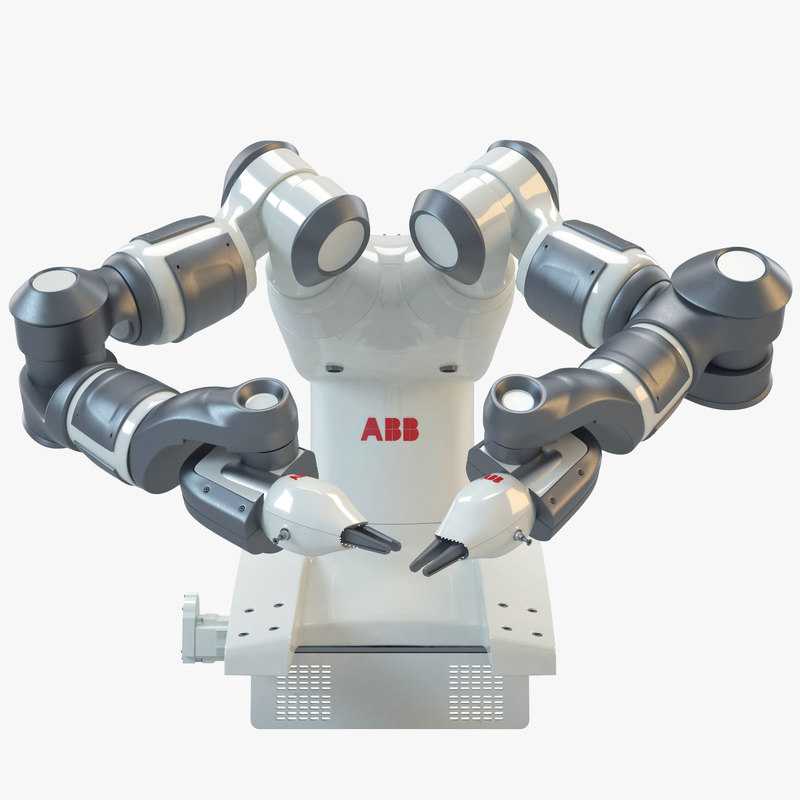
\includegraphics[width=7.0cm]{./gfx/yumi}
               \caption{Picture of a Collaborative Robot \cite{abb2017}.}
               \label{fig:chapteroutline}
\end{figure}

  % Chapter 1 Introduction
\cleardoublepage 
\chapter{Methodology}
 \label{chapter:rapproach}
 

 
The methodology chapter describe and explain the research methods, techniques, and procedures you used to conduct your study. It serves as a roadmap for how you gathered and analyzed data, enabling other researchers to understand and potentially replicate your work.



\section{Considerations}
As you develop this chapter, the title could be one of the following: 1. Method, 2. Methodology, 3. Methodological Approach.
Consider these points in this chapter:

\begin{enumerate}

\item Research Philosophy and Approach:

\begin{inparaenum}
\item Start by explaining your research philosophy or paradigm (e.g., positivism, interpretivism) and approach (\eg~deductive, inductive).
\item Justify your choice of philosophy and approach, explaining why they are appropriate for your research.
\end{inparaenum}



\item Research Design:

	\begin{inparaenum}
	\item Describe the overall research design or framework of your study (\eg experimental, survey, case study, qualitative, quantitative).
	\item Justify your choice of philosophy and approach, explaining why they are appropriate for your research.
	\item Explain why you chose this particular design and how it aligns with your research objectives.
\end{inparaenum}

\item Data Collection Methods:

	\begin{inparaenum}
	\item Detail the methods used to collect data. This might include surveys, interviews, observations, experiments, archival research, etc.
	\item Explain how you selected or recruited participants, if applicable.
	\item Discuss any tools or instruments you used (\eg questionnaires, interview guides).
	\end{inparaenum}

\item Data Analysis Methods:

	\begin{inparaenum}
	\item Describe how you analyzed the collected data. This could involve statistical techniques, content analysis, thematic analysis, or other relevant methods
		\item Justify why these methods were chosen and how they align with your research objectives.	
	\end{inparaenum}
 
 \item Sampling Strategy:
 
	Explain your sampling strategy, including the criteria for participant selection, sample size considerations, and the rationale behind your choice of sample.

\item Ethical Considerations:

	\begin{inparaenum}
	\item Discuss any ethical concerns related to your research, such as informed consent, data privacy, or potential risks to participants.
	\item Explain how you addressed these ethical concerns and obtained necessary approvals or permissions.
	\end{inparaenum}


\item Data Collection Procedures:

 Provide a step-by-step description of how data was collected, including any specific protocols or procedures you followed.

\item Data Validation and Reliability:

 Explain how you ensured the validity and reliability of your data. Discuss any measures taken to reduce bias or errors.

\item Data Management: 

Describe how the collected data was stored, organized, and managed, including any software or tools used for this purpose.

\item Research Timeline (optional):

 If relevant, provide a timeline of when data collection and analysis took place, showing the research's progression.

\item Challenges and Limitations: 

Address any challenges or limitations encountered during the research process, and discuss how you mitigated or managed them.

\item Comparison to Alternative Methods (optional): 

If there were alternative methods that could have been used, briefly discuss why you chose your specific approach over others.
\end{enumerate}

\section{Summary}
The methodology chapter should be written in a clear and detailed manner to enable other researchers to understand and potentially replicate your study. It's also important to ensure that the methodology aligns with your research objectives and research design, providing a strong foundation for the subsequent chapters of your Ph.D. thesis, particularly the data analysis and results chapters.
  
 











 % Chapter 2 Method
\cleardoublepage\chapter{Frame of Reference}
\label{chapter:theory}

In a Ph.D. thesis or any research paper, a \texttt{frame of reference}  typically refers to the theoretical or conceptual framework that serves as a foundation for your study. This framework provides a structure for understanding, interpreting, \& analyzing the research problem and the data or evidence you present. It helps readers \& researchers in your field to contextualize and make sense of your work.


\section{Considerations}
As you develop this chapter, the chapter title can be one of the following: Theory, Theoritical Background, Frame of Reference.
Here are the key aspects of a frame of reference in a Ph.D. thesis:

\begin{enumerate}
\item Theoretical Framework: This involves the theoretical perspectives, concepts, and models that you draw upon to guide your research. It helps you explain and make sense of the phenomena you're investigating.

\item Conceptual Framework: This is a more specific subset of the theoretical framework. It consists of key concepts and relationships that are directly relevant to your research. It provides a structure for analyzing and interpreting your data.

\item Related Literature: The frame of reference often includes a review of relevant literature, which demonstrates how your study is situated within the existing body of knowledge in your field. This literature review helps establish the context and importance of your research.

\item Research Questions or Hypotheses: The frame of reference should connect your theoretical and conceptual framework to your specific research questions or hypotheses. It shows how the established theories and concepts are applied to your study.

\item Justification for Framework Choice: You should explain why you selected this particular frame of reference and how it aligns with your research objectives. What makes it suitable for your study, and why is it the best fit among available alternatives?

\item Methodological Implications: Describe how your frame of reference influences the choice of research methods and data analysis techniques. Theoretical and conceptual frameworks can guide the entire research process.


\item Practical Applications: If applicable, discuss how the knowledge derived from your frame of reference can be practically applied in your field or in solving real-world problems.

\item Limitations and Critiques: Acknowledge any limitations or critiques of your chosen frame of reference. No framework is perfect, and it's essential to recognize its weaknesses.

\end{enumerate}

\section{Summary}
In essence, the frame of reference helps set the intellectual context for your research, and it's a crucial part of any academic work. It provides a roadmap for the reader to understand how you approach your research, which theories or models you rely on, and why your study is relevant and significant within your field.
  % Chapter 3 Theory
\cleardoublepage\chapter{Result}   
\label{chapter:result}
This chapter is where you present the findings of your research complemented by a detailed account of the data, evidence, and outcomes of your study. 

\section{Considerations}
As you develop this chapter, the chapter title can be one of the following: Result, Framework, Case Analysis
Here's what should be included in the results chapter:

\begin{enumerate}

\item Presentation of Data: Display your data in a clear and organized manner. This can include tables, charts, graphs, figures, or any other appropriate visual representations to help readers understand the results.

\item Description of Data: Provide a written description or narrative of the data presented. Explain what the data represents, how it was collected, and any notable characteristics or patterns.


\item Raw Data: In some cases, you may choose to include raw data or transcripts in appendices for readers who want to delve deeper into your findings. However, this is not always necessary and should be considered carefully.

\item Visual Aids: Ensure that visual aids are labeled, appropriately titled, and properly referenced in the text. Make it clear how they relate to your analysis and conclusions.


\item Avoid Interpretation: The results chapter is primarily focused on presenting the data and findings. Avoid interpreting the results in this section; that is the role of the discussion chapter that follows.


\end{enumerate}


\section{Summary}
The results chapter should be a factual and transparent presentation of your findings, allowing readers to draw their own conclusions about the significance of the data. It is in the subsequent discussion chapter that you will provide interpretation, context, and the implications of the results, drawing connections to your research objectives and the existing body of knowledge in your field.

   





 
 


 % Chapter 4 Result
\cleardoublepage\chapter{Discussion} 
\label{chapter:Discussion}
 
This chapter is where you interpret and analyze the results. This chapter allows you to delve into the implications of your findings, discuss their significance, and connect your research to the broader field of study. 

\section{Considerations}

Some considerations for what should be included in the discussion chapter are:

\begin{enumerate}

\item Interpretation of Results: Begin by interpreting the results and explaining their meaning. Discuss the patterns, trends, and relationships you observed in the data. Address any unexpected or contradictory findings and offer possible explanations.

\item Comparison with Previous Research: Analyze how your findings align with or differ from existing literature and research in your field. Discuss how your research contributes to or challenges the current understanding of the topic.

\item Hypotheses or Research Questions: Revisit the hypotheses or research questions you posed in the introduction. Explain whether your results support or reject these statements and what this means for your study.

\item Theoretical Framework: Discuss how your results fit within the theoretical or conceptual framework you introduced in the earlier chapters. Explain how the theory guided your research and what it reveals about the underlying principles.

\item Practical Implications: Explore the practical implications of your findings. How can they be applied in the real world or in your field of study? What are the potential practical benefits or recommendations?

\item Limitations: Acknowledge the limitations of your study. Discuss any constraints, weaknesses, or potential sources of bias that may have affected your results. Honesty about limitations is crucial for maintaining the credibility of your research.

\item Future Research Directions: Propose potential directions for future research based on the gaps or questions that your study has uncovered. What further inquiries or studies could build upon your work?

\item Contributions to the Field: Summarize the contributions your research makes to your field or discipline. Highlight the novel insights, advancements, or changes in understanding that result from your work.

\item Summary and Conclusion: Provide a concise summary of the key points and conclusions drawn from your analysis. Highlight your main contributions.

\item Reflect on the Research Process: Reflect on your research process, including the methods used, data collection, and any challenges you encountered. This can help future researchers understand the practical aspects of conducting similar research.

\end{enumerate}

\section{Summary}

The discussion chapter should offer a clear and thoughtful analysis of your research findings, guiding the reader through your thought process and helping them understand the broader implications of your work. It is a critical component of your thesis, as it demonstrates your ability to synthesize information, critically assess data, and contribute to the body of knowledge in your field.










 % Chapter 5 Discussion
\cleardoublepage\chapter{Conclusion}
\label{chapter:conclusion}

This  chapter serves as the final section of your research document, summarizing and synthesizing the key points, findings, and implications of your study. It offers a sense of closure and provides a clear and concise overview of the entire research project.



\section{Consideration}
Here's what should be included in the conclusion chapter:

\begin{enumerate}


\item Summary of Key Findings: Begin by summarizing the main findings and results of your research. Highlight the most significant and relevant outcomes of your study.

\item Restate the Research Problem: Remind the reader of the specific research problem or questions that your study aimed to address. Restate them clearly and concisely.

\item Review of Research Objectives: Recap the research objectives and goals you set out to achieve at the beginning of your thesis. Explain whether you have met these objectives.

\item Contributions to Knowledge: Discuss the contributions your research has made to the field. Emphasize the novel insights, advancements, or new knowledge generated by your study.

\item Theoretical and Practical Implications: Explain the theoretical and practical implications of your research. How does your work impact the theoretical understanding of the topic, and what are its real-world applications?

\item Limitations: Acknowledge any limitations or constraints in your study, and discuss how they may have influenced the results or the generalizability of your findings.

\item Reflection on Methodology: Reflect on the research methods and methodology used in your study. Discuss the strengths and weaknesses of your approach and any lessons learned for future research.

\item Future Directions: Offer suggestions for future research that could build upon your work. Identify specific areas or questions that remain unanswered or require further investigation.

\item Practical Recommendations (if applicable): If your research has practical applications, provide recommendations for policymakers, practitioners, or relevant stakeholders based on your findings.

\item Personal Reflection (optional): Some researchers choose to include a brief personal reflection on the research process, discussing their own growth, challenges, and insights gained during the study.

\item Final Thoughts and Closing Remarks: End the conclusion chapter with a compelling final thought or statement that leaves a strong impression on the reader and summarizes the significance of your research.


\end{enumerate}

\subsection{Summary}
The conclusion chapter should be concise and focused while still providing a comprehensive overview of the study's major elements. It should leave the reader with a clear understanding of the research's importance, the contributions it has made, and the potential for future research in the field.

\section{Not an Abstract}
The abstract and the conclusion chapter of a Ph.D. thesis serve different purposes and are placed at different points within the document. Here are the key differences between an abstract and the conclusion chapter:

\subsection*{Content}
 
An abstract serves as a condensed summary of the research, highlighting the key aspects of the thesis, including the research problem, objectives, methods, key findings, and conclusions. It does not provide in-depth details.

The conclusion chapter is where the researcher interprets the results, discusses their implications, summarizes the major findings, reflects on the research process, and provides recommendations for further study or practical applications.

\subsection*{Audience}
The abstract is designed to give potential readers a quick understanding of the thesis's content, allowing them to decide whether they want to read the full document. It is often used as a reference when searching for relevant research.

The conclusion chapter is intended for readers who have read the entire thesis and are looking for a thorough understanding of the research's significance and implications

\subsection*{Use}
The abstract is useful for busy researchers who want to assess the relevance of the thesis to their own work or for readers seeking a quick overview of the research without delving into the entire document.

The conclusion chapter is an integral part of the thesis, allowing the researcher to demonstrate their critical thinking and synthesis of the research. It is where the researcher has the opportunity to tie together all the threads of the study and leave the reader with a comprehensive understanding of the research's impact and future directions.

\subsection*{Last Section}
In summary, while both the abstract and the conclusion chapter provide summaries of a Ph.D. thesis, the abstract is a brief, initial overview intended for a broad audience, while the conclusion chapter is a more detailed and comprehensive analysis and reflection, serving as the closing section for those who have read the entire document. % Chapter 6 Conclusion



\iffalse

====
DONE

Title Page - V1 2023-10-15
Back Page - V1 2023-10-15
Dedication - V1 2023-10-15
Abstract - What is an abstract? - V1 2023-10-15
Acknowledgement - V1 2023-10-15
Appended Articles - V1 2023-10-15


2023-10-17 - in the TOC the list of figures, definitions etc. is very big typeface. Not good. Can comment it off.
TOC  
Definitions 
Acronyms
List of figures
List of tables

Configuration file cleanup
style file clean up




Chapters - 1
Introduction  
 References
 figures, tables, headings 

Chapter - 2
Methodology



Chapter - 3 theory
  
Chapter - 4 - result 

Chapter 5 - Discussion
====

Chapter 6 - Conclusion


References.

Spikblad 

The page between the main article and the appended articles

Appended article template. this is for the articles orginally published and that will be included in the thesis.



-- double check this works in both ubuntu and windows. How? virtual machies x2 
-- Fresh install for both windows and Ubuntu and scientificLinux

Clean Pdf, tex files, Folder


* See others
\fi




%\afterpage{\null\newpage} % used to move one page
 


%----------------------------------------------------------------------------------------
%	POST-CONTENT THESIS PAGES
%----------------------------------------------------------------------------------------
\cleardoublepage% Bibliography

\label{app:bibliography} % Reference the bibliography elsewhere with \autoref{app:bibliography}
\renewcommand\bibname{References}
\manualmark
\markboth{\spacedlowsmallcaps{\bibname}}{\spacedlowsmallcaps{\bibname}} 
\refstepcounter{dummy}
 
\addtocontents{toc}{\protect\vspace{\beforebibskip}} % Place the bibliography slightly below the rest of the document content in the table of contents
\addcontentsline{toc}{chapter}{\tocEntry{\bibname}}




\bibliographystyle{unsrt}

%\bibliography{C:/Users/vargo61/Dropbox/Papers/Literature_LatexBIB/varunbib_2018} 
\bibliography{phdthesis} 


 
 
% To add appended articles to your thesis pdf file. 

\pagenumbering{gobble}
\phantomsection
%\addcontentsline{toc}{chapter}{} %\Rmnum{1} -- \Rmnum{9}
%\phantomsection
\addcontentsline{toc}{chapter}{Appended Articles} %\Rmnum{1} -- \Rmnum{9}
\addcontentsline{toc}{section}{Paper \Rmnum{1}\dots\dots 101 -- 110}
\addcontentsline{toc}{section}{Paper \Rmnum{2}\dots\;\;\;201 -- 210}



 % Bibliography


%----------------------------------------------------------------------------------------
%	THESIS CONTENT - APPENDICES
%----------------------------------------------------------------------------------------
\cleardoublepage




\end{document}
